Mit Hilfe der, in Abbildung \ref{Versuchsaufbau<1} gezeigten Apparatur, sollte die Dampfdruckkurve für $p\leq \SI{1}{\bar}$ bestimmt werden.
\begin{figure}[h!]
	\centering
	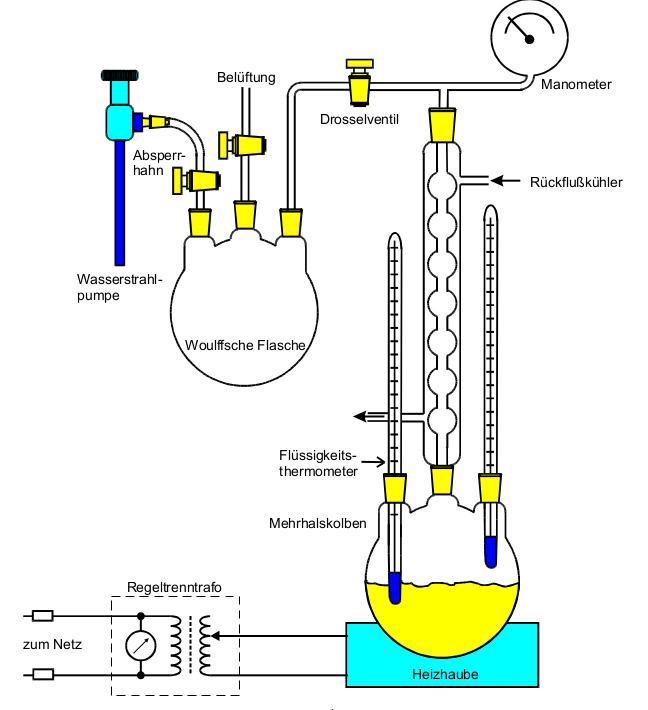
\includegraphics[width=0.9\textwidth]{Versuchsaufbau<1Bar.png}
	\caption{Versuchsaufbau für die Messung der Dampfdruckkurve bei $p<\SI{1}{\bar}$\cite{V203}}
	\label{Versuchsaufbau<1}
\end{figure} \\
Nach dem Evakuieren des Mehrhalskolbens, wurde das darin enthaltene Wasser erhitzt. Sobald das Wasser anfing zu verdampfen, wurden der Druck im Kolben mit einem digitalen Messgerät und die Temperatur des Dampfes mit einem Flüssigkeitsthermometer in $\SI{5}{\celsius}$-Schritten bis zur Siedetemperatur gemessen. \\
\newpage
Abbildung \ref{Versuchsaufbau>1} zeigt die Messapparatur, mit der die Dampfdruckkurve für $p \geq \SI{1}{\bar}$ gemessen wurde. Zunächst wurde der Kolben inklusive dem darin enthaltenen Wasser bei konstantem äußerem Druck erhitzt. Bei Temperaturen im Bereich $\SI{94}{\celsius}\leq T\leq\SI{130}{\celsius}$ wurde der zugehörige Druck abgelesen.
\begin{figure}
	\centering
	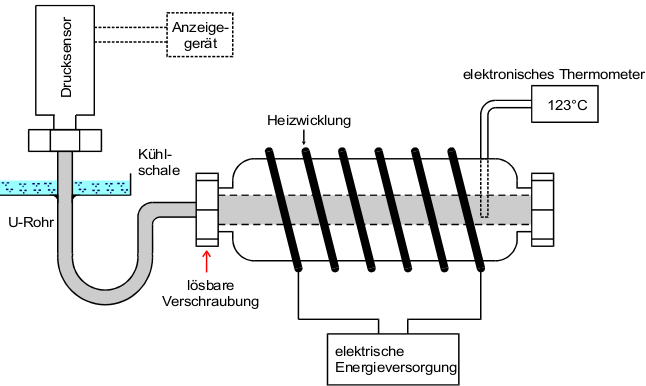
\includegraphics[width=0.8\textwidth]{Versuchsaufbau>1Bar.png}
	\caption{Versuchsaufbau für die Messung der Dampfdruckkurve bei $p\geq\SI{1}{\bar}$\cite{V203}}
	\label{Versuchsaufbau>1}
\end{figure}
Bei der späteren Berechnung ist zu beachten, dass das Druckmanometer nicht richtig geeicht war, sodass für alle Werte gilt
\begin{equation}
	p(T) = p_\text{gemessen}(T) - (p_\text{gemessen}(\SI{100}{\celsius})-\SI{10e+5}{\pascal}).
\end{equation}